

\chapter{Projeto do Sistema}

Este capítulo tem o propósito de transformar as prévias ilustrações e representações em uma especificação mais detalhada e técnica, assim estabelece mais detalhes sobre os recursos e tecnologias que foram adotadas.

\section{Arquitetura do Sistema}
\begin{figure}[H]
	\caption{\label{fig_comp}Diagrama de Componentes}
	\begin{center}
	    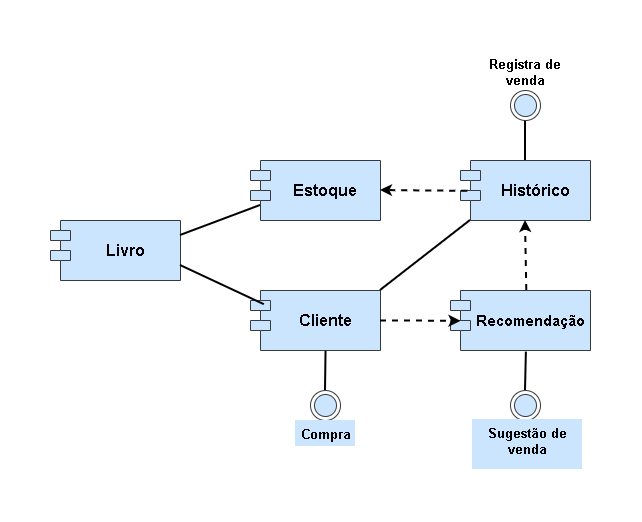
\includegraphics[scale=0.5]{imagens/diag_comp.png}
	\end{center}
\end{figure}

\section{Projeto dos Componentes}
Em nível arquitetural, em suma, a solução é formada dos 5 componentes: livro, estoque, cliente, histórico e recomendação. Como uma livraria, o componente Livro é importante pois forma o catálogo e é envolvido nas vendas, o Estoque mantém informação dos livros e suas quantidades, o Cliente pode ser registrado para vendas futuras, o Histórico registra vendas de clientes salvos e a Recomendação usa esse registro tanto quanto o catálogo para sugerir livros também em vendas futuras.

\section{Modelo de Dados}
O modelo mais avançado desenvolvido para a camada de dados é o contemplado na próxima figura, no entanto, para o contexto dessa primeira parte do projeto, ele se encontra incompleto. Portanto, considera-se para presentes protótipos e desenvolvimento apenas o modelo simplificado.
\begin{figure}[H]
	\caption{\label{fig_mer}Modelagem de Dados}
	\begin{center}
	    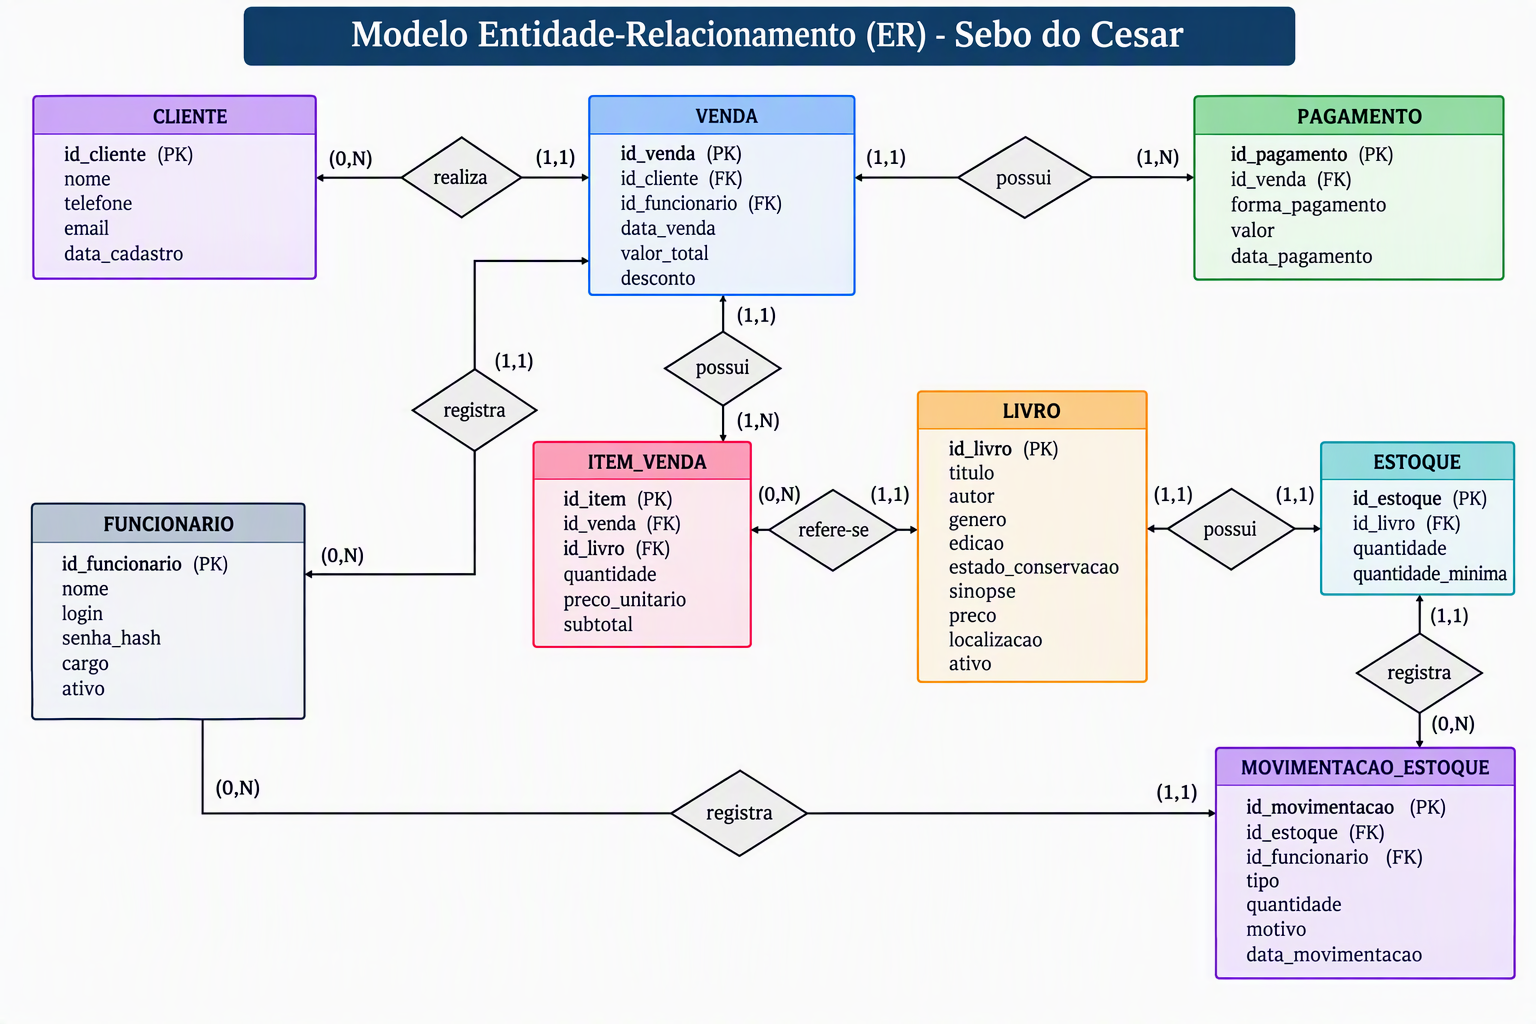
\includegraphics[scale=0.4]{imagens/mer.png}
	\end{center}
\end{figure}

\begin{figure}[H]
	\caption{\label{fig_mer-simp}Modelo Simplificado}
	\begin{center}
	    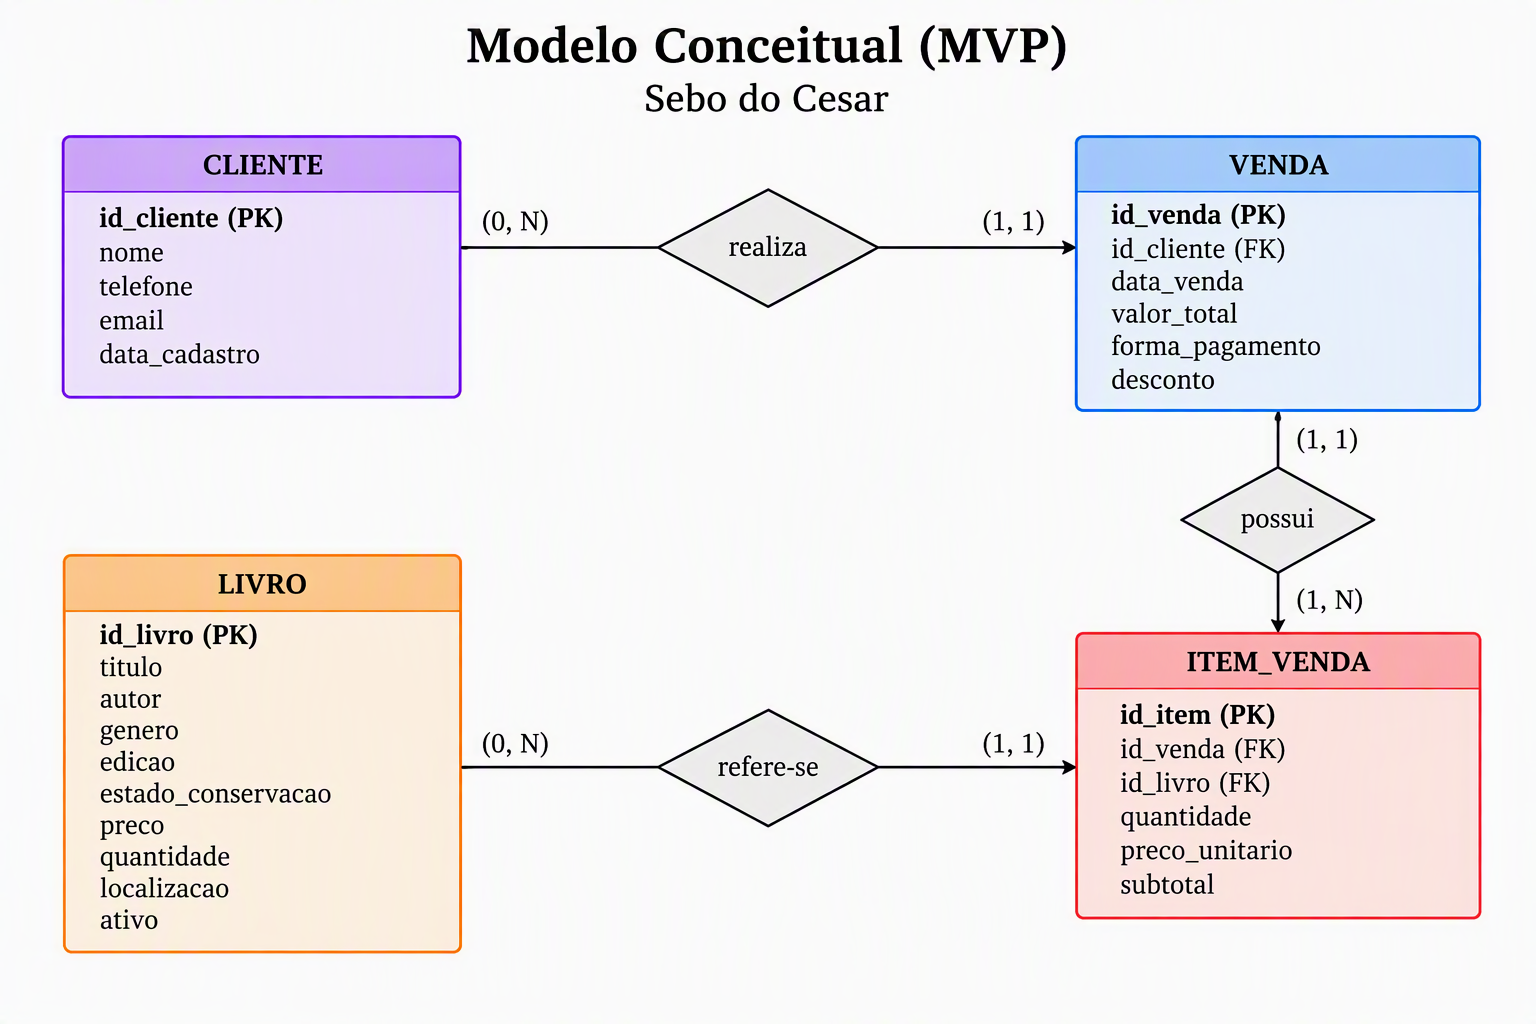
\includegraphics[scale=0.4]{imagens/mer_simp.png}
	\end{center}
\end{figure}

\subsection{Relacionamento entre Cliente e Venda}

\noindent\textbf{Cardinalidade:} \texttt{CLIENTE (0,N) ---- realiza ---- (1,1) VENDA}

\noindent Leitura:
\begin{itemize}
  \item Um \textbf{cliente} pode realizar nenhuma ou várias vendas.
  \item Cada \textbf{venda} deve estar associada a exatamente um cliente.
\end{itemize}

\subsection{Relacionamento entre Venda e Item de Venda}

\noindent\textbf{Cardinalidade:} \texttt{VENDA (1,1) ---- possui ---- (1,N) ITEM\_VENDA}

\noindent Leitura:
\begin{itemize}
  \item Cada \textbf{ITEM\_VENDA} pertence a exatamente uma VENDA.
  \item Uma \textbf{VENDA} deve possuir um ou vários itens de venda.
\end{itemize}

\subsection{Relacionamento entre Livro e Item de Venda}

\noindent\textbf{Cardinalidade:} \texttt{LIVRO (0,N) ------ refere-se ------ (1,1) ITEM\_VENDA}

\noindent Leitura:
\begin{itemize}
  \item Um \textbf{LIVRO} pode aparecer em nenhum ou em vários ITENS\_VENDA.
  \item Cada \textbf{ITEM\_VENDA} deve referenciar exatamente um LIVRO.
\end{itemize}

\section{Projeto da Interface do Usuário}
O sistema será composto de 5 interfaces que precisam de uma autenticação anterior. A tela inicial dispõe de um dashboard com alertas e uma visão geral do estoque, os outros menus compreendem um catálogo que exibe todo livro e seus detalhes, um registro de clientes e um registro de vendas realizadas relacionadas a cada cliente e, por fim, uma página que soma a esse segundo registro, onde propriamente registra-se cada venda.

\section{Diagramas de Interação}
O acesso e a saída do usuário marcam o início e o fim de todo processo realizado na aplicação. Conforme o front-end cuida da camada de apresentação, são necessários ocasionalmente dados oriundos do banco e dependendo do contexto, uma parte do controle, realizada também no lado cliente, toma parte no fluxo dessas requisições. Como se vê na representação a seguir, menus do sistema se alternam na sequência das ações.
\begin{figure}[H]
	\caption{\label{fig_seq}Diagrama de Sequência}
	\begin{center}
	    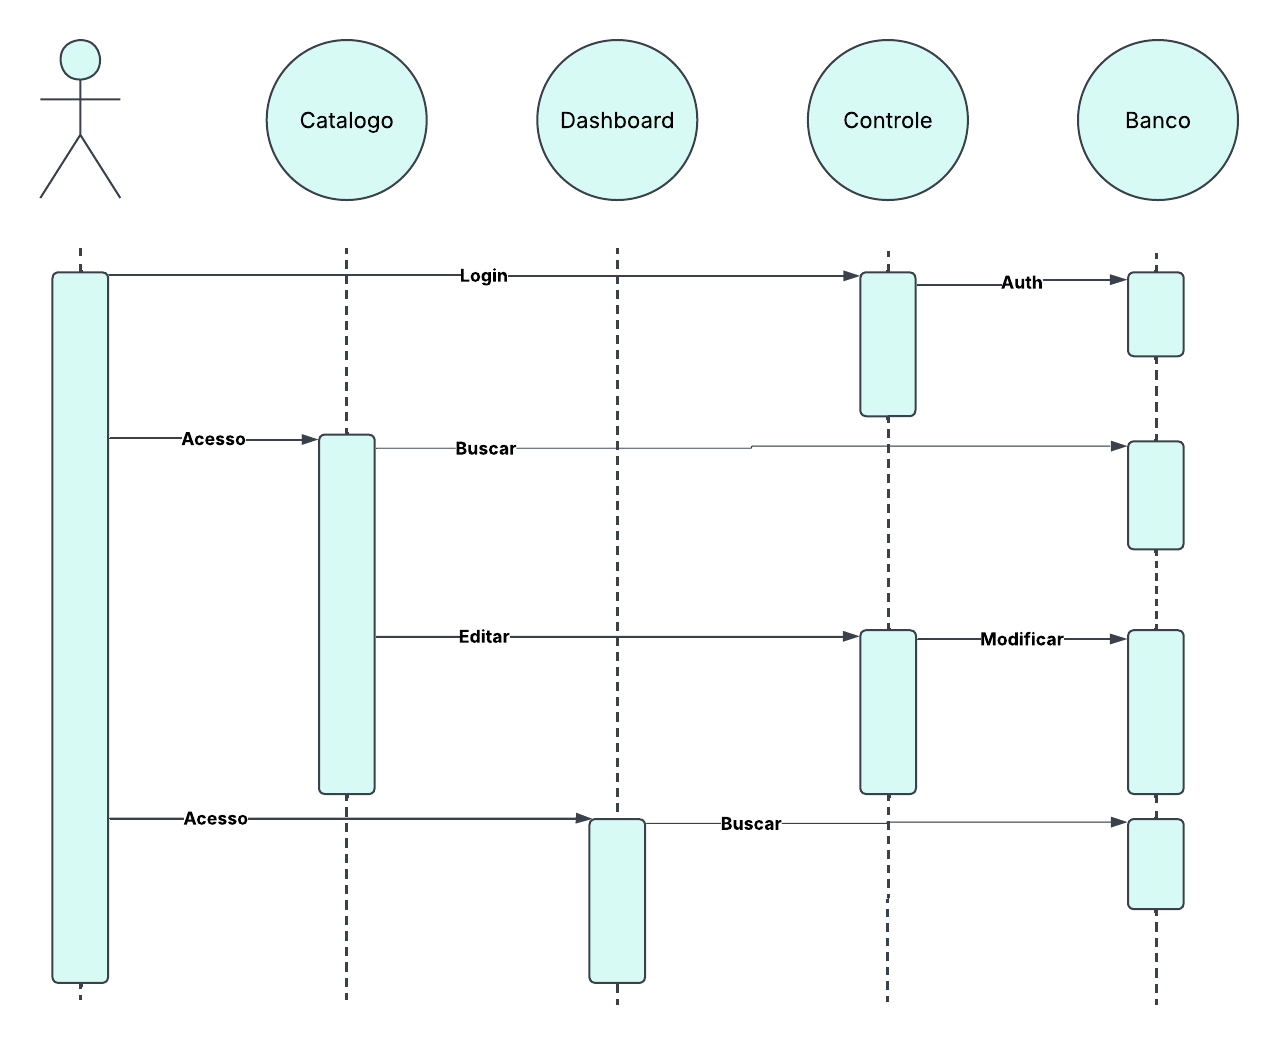
\includegraphics[scale=0.7]{imagens/diag_seq.png}
	\end{center}
\end{figure}

\section{Tecnologias Utilizadas}
As linguagens definidas neste projeto de software foram Javascript com o framework React \cite{react} na camada de apresentação e parte de lógica, Python para a camada de lógica de programação e integração e a estrutura SQLite para a camada de dados. Para a geração deste documento por si, é utilizado o sistema de preparação de documentos LaTex \cite{latex}.

\section{Segurança e Controle de Acesso}
A segurança do sistema é estruturada a partir de um mecanismo centralizado na autenticação inicial, responsável por validar as credenciais do usuário no momento do primeiro acesso à aplicação. Adota-se um nível de encapsulamento simples baseado nos protocolos web tradicionais. A autorização é gerenciada de forma direta com base no perfil associado ao usuário autenticado e a segurança dos dados em trânsito é garantida pela utilização de protocolos como o HTTPS e recursos dos frameworks usados.
\begin{figure}[H]
	\caption{\label{fig_est}Diagrama de Estado}
	\begin{center}
	    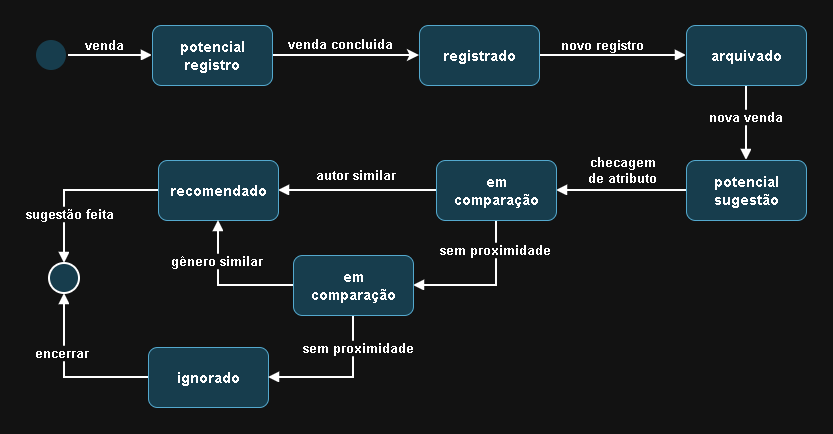
\includegraphics[scale=0.5]{imagens/diag_estado.png}
	\end{center}
\end{figure}